% Beamer Biz
\documentclass[final]{beamer}
\usepackage[scale=1.25]{beamerposter} % Use the beamerposter package for laying out the poster
\usetheme{confposter} % Use the confposter theme supplied with this template
\setbeamercolor{block title}{fg=ngreen,bg=white} % Colors of the block titles
\setbeamercolor{block body}{fg=black,bg=white} % Colors of the body of blocks
\setbeamercolor{block alerted title}{fg=white,bg=dblue!70} % Colors of the highlighted block titles
\setbeamercolor{block alerted body}{fg=black,bg=dblue!10} % Colors of the body of highlighted blocks

%-----------------------------------------------------------
% Define the column widths and overall poster size
% To set effective sepwid, onecolwid and twocolwid values, first choose how many columns you want and how much separation you want between columns
% In this template, the separation width chosen is 0.024 of the paper width and a 4-column layout
% onecolwid should therefore be (1-(# of columns+1)*sepwid)/# of columns e.g. (1-(4+1)*0.024)/4 = 0.22
% Set twocolwid to be (2*onecolwid)+sepwid = 0.464
% Set threecolwid to be (3*onecolwid)+2*sepwid = 0.708

\newlength{\sepwid}
\newlength{\sepwidtwo}
\newlength{\onecolwid}
\newlength{\onecolwidtwo}
\newlength{\halfcolwid}
\newlength{\halfcolwidtwo}
\newlength{\threecolwid}
\setlength{\paperwidth}{56in} % A0 width: 46.8in
\setlength{\paperheight}{37in} % A0 height: 33.1in
\setlength{\sepwid}{0.025\paperwidth} 
\setlength{\sepwidtwo}{0.02\paperwidth} % Separation width (white space) between columns
\setlength{\onecolwid}{0.25\paperwidth} % Width of one column
\setlength{\onecolwidtwo}{0.4\paperwidth} % Width of one column
%\setlength{\onecolwidthree}{0.3\paperwidth} % Width of one column
\setlength{\halfcolwid}{0.125\paperwidth} % Width of one column
\setlength{\halfcolwidtwo}{0.19\paperwidth} % Width of one column
%\setlength{\twocolwid}{0.464\paperwidth} % Width of two columns
%\setlength{\threecolwid}{0.708\paperwidth} % Width of three columns
\setlength{\topmargin}{-0.5in} % Reduce the top margin size
%-----------------------------------------------------------
\usepackage{graphicx}

\usepackage{booktabs} % Top and bottom rules for tables

\title{A Markov Model for Analysis of Musical Genre} % Poster title

\author{John O. Brickley\footnote{jobrickley@alaska.edu, Department of Philosophy}, Wolfgang Olsson\footnote{wqolsson@alaska.edu, Department of Music (Minor)}, and Martin Cenek\footnote{mcenek@uaa.alaska.edu, Department of Computer Science and Engineering}}

\begin{document}

\addtobeamertemplate{block end}{}{\vspace*{2ex}} % White space under blocks
\addtobeamertemplate{block alerted end}{}{\vspace*{2ex}} % White space under highlighted (alert) blocks

\setlength\belowcaptionskip{0ex} % White space under figures
\setlength\belowdisplayshortskip{0ex} % White space under equations

\begin{frame}[t] % The whole poster is enclosed in one beamer frame

\begin{columns}[t] % The whole poster consists of three major columns, the second of which is split into two columns twice - the [t] option aligns each column's content to the top

\begin{column}{\sepwid}\end{column} % Empty spacer column

\begin{column}{\onecolwid} % The first column

\begin{alertblock}{Hypothesis}
We hypothesize that `flattening' of pieces of music to linear sequences of notes while tallying occurrences of each pair will yield probabilistic transition matrices enabling automated grouping of analyzed pieces into established musical genres.
\end{alertblock}

\begin{column}{\onecolwid} % Approach column
\begin{block}{Approach}
\begin{enumerate}
\item Assembled a corpus of classical, gospel, and folk music for analysis.
\item Processed selected pieces to produce a list of note letters.
\item Generated matrices of each note-pair's occurrence.
\item Calculated mean square error for each pair of matrices.
\item Created a force-directed graph with clustering of pieces inversely proportional to mean square error.
\item Checked against hypothesis.
\end{enumerate}
\end{block}
\end{column}


\begin{columns}[t]

\begin{column}{\halfcolwid}
\begin{block}{Advantages}
\begin{itemize}
\item Quantification of similarity between pieces of music.
\item Analysis independent of external data sets.
\item Domain agnostic approach with potential applications in other fields.
\end{itemize}
\end{block}
\end{column}

\begin{column}{\halfcolwid}
\begin{block}{Disadvantages}
\begin{itemize}
\item Factorial growth in number of comparisons between pieces may lead to computational inefficiency.
\item Exclusion of potentially relevant features from analysis. 
\end{itemize}
\end{block}
\end{column}
\end{columns}

\begin{column}{\onecolwid}
\begin{block}{Transition Matrices}
The probability of each note-pair's occurrence was calculated and these probabilities were input to a $12\times12$ matrix where rows were first- and columns were second-notes in each pair. 
\begin{figure}
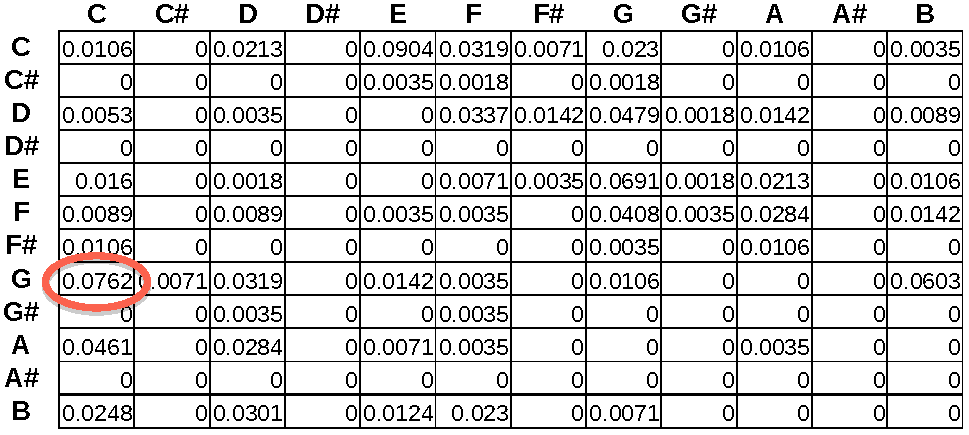
\includegraphics[width=\halfcolwidtwo]{Visuals/WTK1transitionmat.pdf}
\caption{Transition matrix for Das Wohltemperierte Klavier Prelude No. 1}
\end{figure}
\end{block}
\end{column}

\end{column} % End of the first column

\begin{column}{\sepwid}\end{column} % Empty spacer column

\begin{column}{\onecolwidtwo} % (column 2)
\begin{columns}[t]

\begin{column}{\halfcolwidtwo}

\begin{block}{Flattening}
\begin{enumerate}
\item{Pieces were transposed to a common key (C) to ease comparison.}
\begin{figure}

\includegraphics[width=1\halfcolwidtwo]{Visuals/WTK10.pdf}
\caption{One of the pieces which was processed.}
\end{figure}
\item{Notes from each piece were then extracted and arranged in a list ordered according to time, pitch, and other features such as accidentals. For example, the notes in Figure \ref{wtk1} were converted to the list \emph{C, E, G, C, E, G, C, E, C, E, G, C, E, G, C, E, E}.}
\begin{figure}
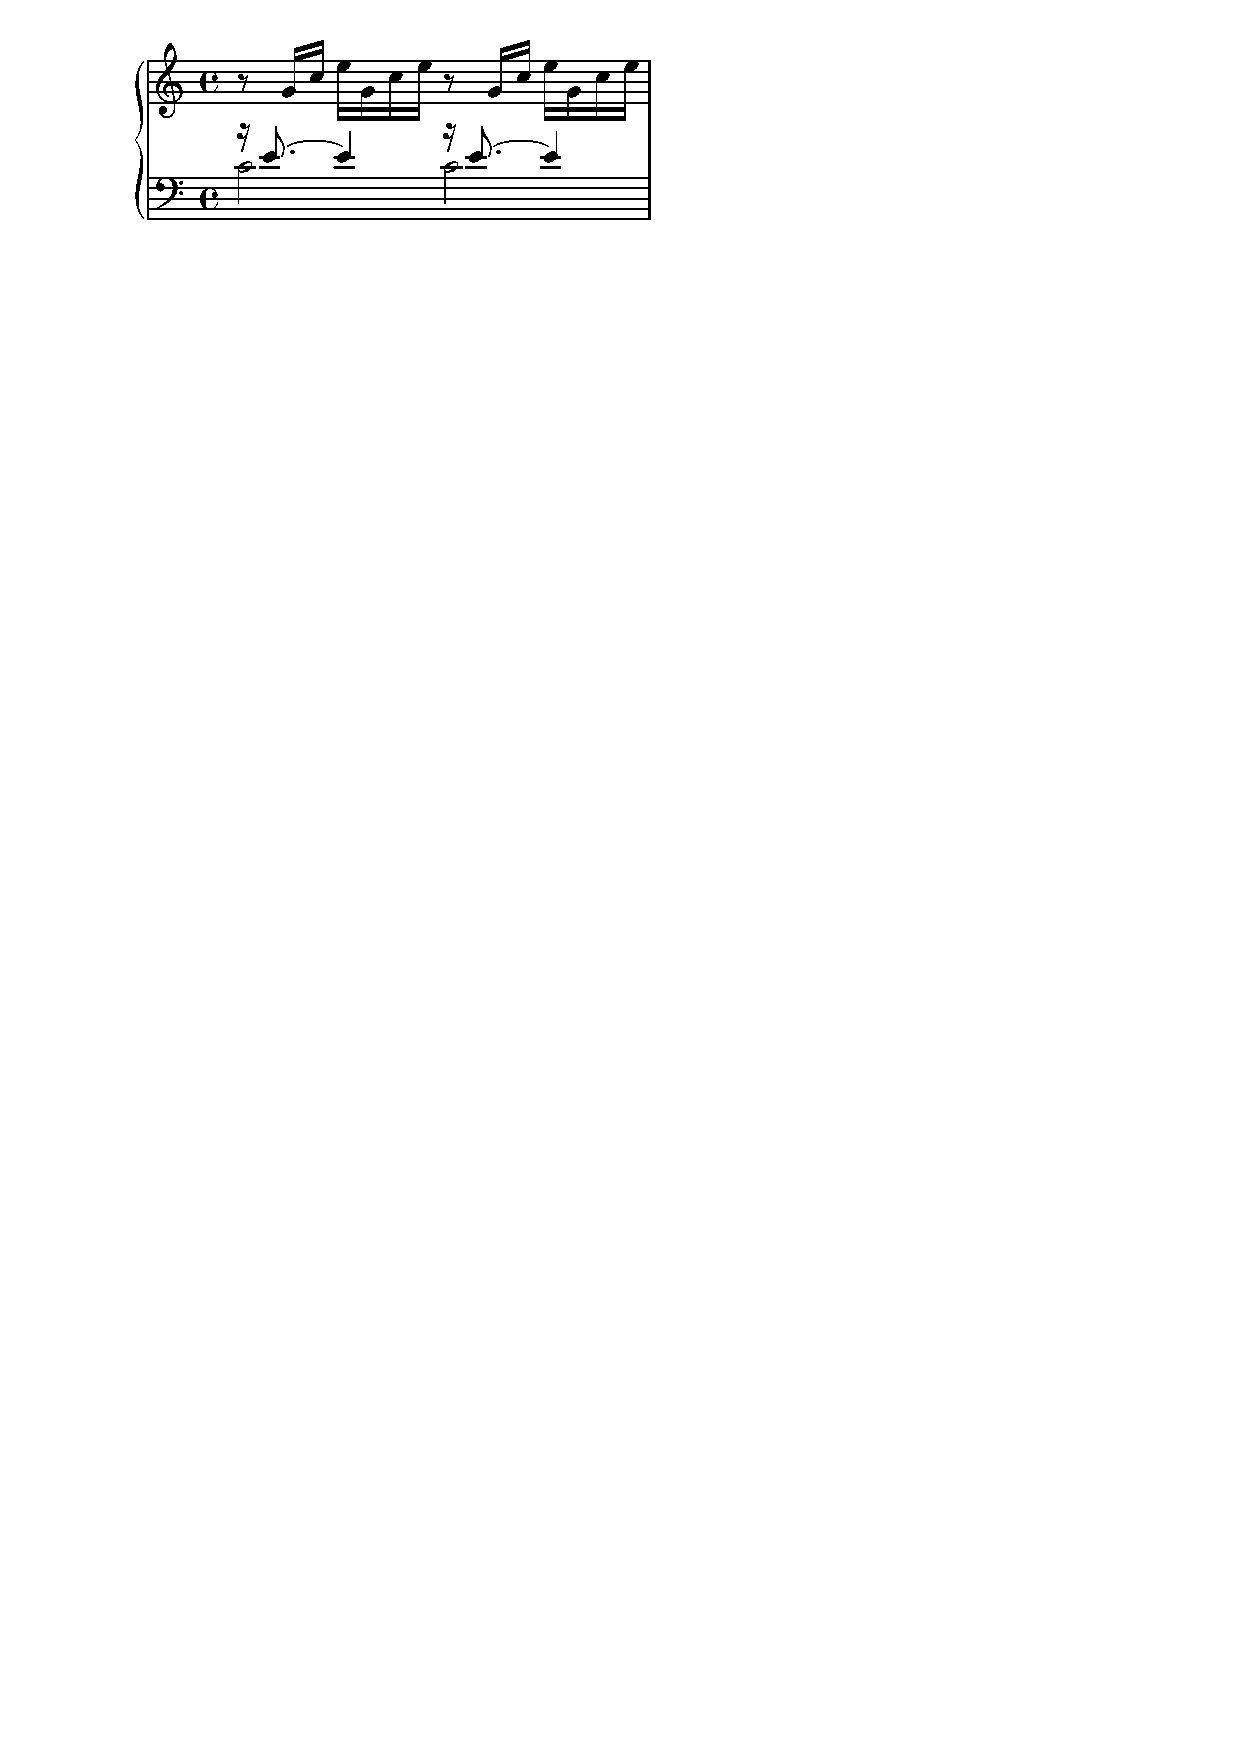
\includegraphics[width=1\halfcolwidtwo]{Visuals/WTK1.pdf}
\caption{A transposed, but unflattened section.}
\label{wtk1}
\end{figure}
\end{enumerate}
\end{block}

\end{column}

\begin{column}{\sepwidtwo}\end{column} % Empty spacer column

\begin{column}{\halfcolwidtwo}

\vskip2in
\begin{block}{Network Graph}
Preliminary graphs such as that shown in Figure \ref{graph} have been generated for small corpora of music. The network graph shows clustering between similar pieces and distance between dissimilar pieces, which supports our hypothesis.
\end{block}

\vskip1.5in
\begin{block}{Results \& Analysis}
The results of the analysis recapitulated accepted genre classifications. In Wohltemperierte Klavier Prelude No. 1, for example, the analysis matched the expected high density of G-C, C-E, and E-G transitions. Furthermore, in A North Country Maiden (ANCM) there was a high probability of transition between elements of the Dominant and Tonic chords. From this we conclude that the preliminary model correctly generated the transition tables which confirm common knowledge of music theory. 
\end{block}
\end{column}
\end{columns}

\begin{column}{\onecolwidtwo}
\begin{block}{Selected References}

[1]	J. C. Gonz\~{a}lez-Avella, V. M. Egu\'iluz, M. G. Cosenza, K. Klemm, J. L. Herrera, and M. S. Miguel. Local versus global interactions in nonequilibrium transitions: A model of social dynamics. Physical Review, 73, 2006.

[2]	R. Axelrod. The dissemination of culture: A model with local convergence and global polarization. The Journal of Conflict Resolution, 41(2):203-226, April 1997.

[3]	J. H\aa kansson and W. Nordstr\"om. Finding clusters of similar artists: analysis of dbscan and k-means clustering. April 2012.

[4]	B. Jurish. bang: Pure Data, chapter Music as a Formal Language. First edition, 2006.

[5]	G. E. Poliner and D. P. Ellis. A classification approach to melody transcription. In ISMIR 2005: 6th International Conference on Music Information Retrieval: Proceedings: Variation 2: Queen Mary, University of London \& Goldsmiths College, University of London, 11-15 September, 2005, pages 161-166. Queen Mary, University of London, 2005.

\end{block}
\end{column}

\end{column} % End of 2

\begin{column}{\sepwid}\end{column} % Empty spacer column

\begin{column}{\onecolwid} % (column 3)

\begin{figure}
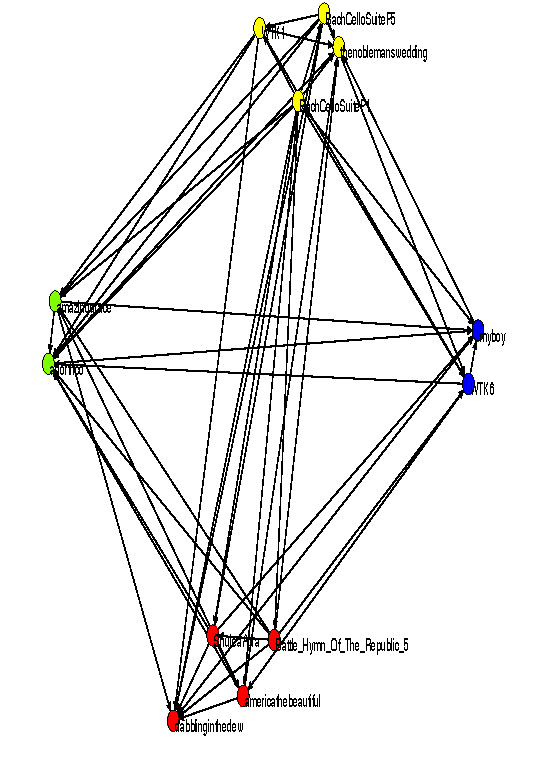
\includegraphics[width=1\onecolwid, height=.66\onecolwid]{Visuals/clippedgraph.pdf}
\caption{An example network graph for a small corpora of pieces.}
\label{graph}
\end{figure}
\vskip2in\begin{alertblock}{Conclusions}
\begin{itemize}
\item Automatic detection of high-level features such as genre in music is possible, even given relatively small data sets.
\item This model has the ability to recognize features common to established musical genres.
\item The techniques used may also prove useful in fields such as linguistics, especially in areas such as fine-grained Sociolinguistic Dialect analysis and classification.
\end{itemize}

\end{alertblock}
\begin{block}{Acknowledgements}
    We would like to acknowledge Brendan Babb, of UAA's Computer Science and Mathematics departments, whose assistance with this project proved invaluable. Additionally, we thank the maintainers of the Music21 and Natural Language Toolkit libraries for the Python language.
\end{block}

\end{column} % End of column 3

\end{columns} % End of all the columns in the poster

\end{frame} 

\end{document}
